\section{The performance-complexity trade-off problem}\label{sec:performance-complexity}

The main aim of this work is to explore the performance-complexity characteristics in the context of graph learning, as introduced in \cite{prochazka_downstream_2022}. Consider an undirected graph \( G \) with nodes \( V \left( G \right) \) and edges \( E \left( G \right) \). The result of the graph coarsening part of the algorithm is a sequence of graphs \( G_0, G_1, G_2, \dots, G_L \) where \( G_0 = G \) and \( L \in \mathfield{N} \) is a hyper-parameter of the method.
Given a model \( M \) that operates on graphs, a performance metric, and a complexity metric, the sequence \( G_0, G_1, \dots, G_L \) corresponds to points in the performance-complexity plane, where the original graph \( G_0 \) usually provides the best performance and incurs the most complexity and subsequent coarsened graphs improve complexity and hurt performance. -- see Figure~\ref{fig:performance-complexity} for an illustration.

\begin{figure}
  \centering
  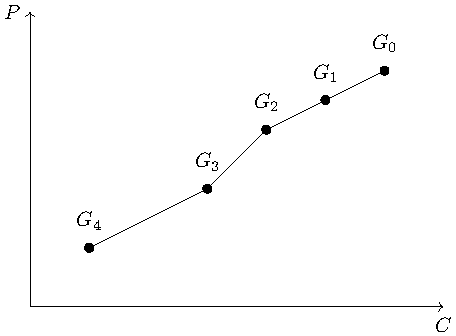
\includegraphics[width=0.35\textwidth]{images/performance-complexity/performance-complexity.pdf}
  \caption{An example of a performance-complexity curve for a sequence of graphs.}
  \label{fig:performance-complexity}
\end{figure}

This performance-complexity characteristic allows for a choice of an optimal \textbf{working point} for the model M -- i.e., the choice of the optimal coarsening level \( G_i \), which directly influences both the performance and the complexity of the model. The choice of the working point, suitable performance metric and complexity metric are subjective and depend on the particular use-case, downstream task and the environment in which the model is to be deployed. In this work, the transductive node classification accuracy on a testing dataset is chosen as the performance metric. For the complexity metric, the number of nodes in the graph was chosen as it constitutes a good proxy for real-world algorithmic complexity, as shown in \cite{chiang_cluster-gcn_2019}.

\subsection{Computational complexity of finding the optimal working point}

While the methods proposed in the rest of this work may yield models and graphs with lower computational demands than models using the original graph, the algorithm for finding the optimal working point itself entails running the same complex models on multiple graphs, therefore potentially offsetting any gains from the lower complexity of the model itself. To overcome these potential shortcomings, the following options are considered:
\begin{itemize}
  \item The optimal working point may generalize to datasets other than the one used for the performance-complexity analysis, for example when collecting data from the same source periodically.
  \item The whole performance-complexity curve is not needed to choose the optimal working point. In the context of this work, the graphs are evaluated in reverse order, i.e. starting with \( G_L \). As such, the evaluation only needs to be run until reaching a working point that is acceptable for the intended use-case.
\end{itemize}
Further discussion of performance and complexity metrics, their suitability and the practical usefulness is considered in \cite{prochazka_downstream_2022}.
